\documentclass[border=5pt]{standalone}
\usepackage{tikz}
\usetikzlibrary{arrows,snakes,backgrounds,patterns,shapes.geometric,calc}

\begin{document}

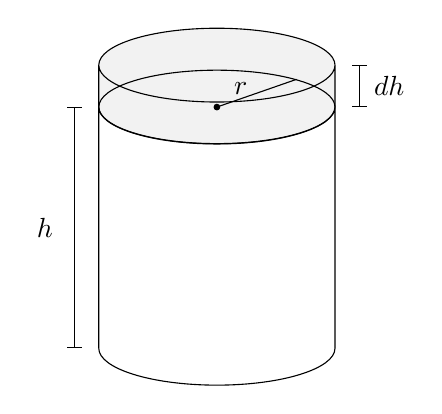
\begin{tikzpicture}[scale=1]
    \node [draw, cylinder, cylinder uses custom fill, cylinder body fill=lightgray!20, cylinder end fill=lightgray!20, shape aspect=4, rotate=90, minimum width=3cm] (c1) at (0,1.8){};

    \coordinate(dhtop) at ($(c1.after top)!-1*.1!(c1.before top)$);
    \coordinate(dhbot) at ($(c1.before bottom)!-1*.1!(c1.after bottom)$);
    \coordinate(dhlabel) at ($(dhtop)!.5!(dhbot)$);
    \draw[|-|] (dhbot)--(dhtop);
    \path (dhlabel) node[right, outer sep = 2pt] {$dh$};

    \node [draw, cylinder, shape aspect=4, rotate=90, minimum height=4cm, minimum width=3cm] (c) {};

    \coordinate(htop) at ($(c.before top)!-1*.1!(c.after top)$);
    \coordinate(hbot) at ($(c.after bottom)!-1*.1!(c.before bottom)$);
    \coordinate(hlabel) at ($(htop)!.5!(hbot)+(c.north)!.9!(c.center)$);

    \draw[|-|] (hbot)--(htop);
    \path (hlabel) node[left] {$h$}; %Modify height label here

    \coordinate (center) at ($(c.before top)!0.5!(c.after top)$);
    \filldraw (center) circle (1pt);

    \coordinate (rlabel) at ($(center) !0.5!(c.after top)$);
    \coordinate (rtop) at ($(center)!-1*.1!(c.after top)$);

    \coordinate (rend) at ($(c.mid east)!0.5!(c.after top)$);
    \draw[-, shorten >=-10] (center) -- (rend);
    \path (rend) node[outer sep = 5pt, left] {$r$};
\end{tikzpicture}

\bigskip

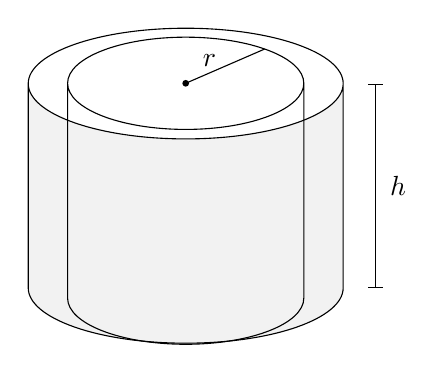
\begin{tikzpicture}[scale=1]
    \node [draw, cylinder, shape aspect=6, rotate=90, cylinder uses custom fill, cylinder body fill=lightgray!20, minimum height=4cm, minimum width=4cm] (c1) at (0,0){};

    \coordinate(htop) at ($(c1.after top)!-1*.1!(c1.before top)$);
    \coordinate(hbot) at ($(c1.before bottom)!-1*.1!(c1.after bottom)$);
    \coordinate(hlabel) at ($(htop)!.5!(hbot)$);
    \draw[|-|] (hbot)--(htop);
    \path (hlabel) node[right, outer sep = 2pt] {$h$};

    \node [draw, cylinder, shape aspect=5, rotate=90, minimum height=3.9cm, minimum width=3cm] (c) {};

    \coordinate (center) at ($(c.before top)!0.5!(c.after top)$);
    \filldraw (center) circle (1pt);

    \coordinate (rlabel) at ($(center) !0.5!(c.after top)$);
    \coordinate (rtop) at ($(center)!-1*.1!(c.after top)$);

    \coordinate (rend) at ($(c.mid east)!0.5!(c.after top)$);
    \draw[-, shorten >=-10] (center) -- (rend);
    \path (rend) node[outer sep = 5pt, left] {$r$};
\end{tikzpicture}

\end{document}
